\documentclass[a4paper,10pt,twocolumn]{article}
%\documentclass[a4paper,10pt]{article}
\usepackage[pdftex]{graphicx}
\usepackage{float}
\usepackage{times}
\usepackage{color}
%\usepackage{fancyheadings}
%\restylefloat{figure}

%\oddsidemargin=0.1in
\topmargin=-0.8in
\textheight=9.8in
\textwidth=6.25in

\parskip 10pt
\parindent 0in

%\parskip 0pt
%\parindent 0.25in
\newif\ifdraft
%\drafttrue


\ifdraft
\newcommand{\fixme}[1]{ { \bf{ ***FIXME: #1 }} }
\newcommand{\jhanote}[1]{ {\textcolor{red} { ***Jha: #1 }}}
\else
\newcommand{\jhanote}[1]{}
\newcommand{\fixme}[1]{}
\fi


\begin{document}
\thispagestyle{plain}
\title{Distributed High Performance Computing \\ using SAGA}
\title{Using Interoperable Loosely Coupled Applications for HIV-1 Protease Simulation}
\author{Owain~A.~Kenway\footnotemark, Shantenu~Jha\footnotemark, David~Wright\footnotemark, Joohyun~Kim\footnotemark, Peter~V.~Coveney\footnotemark \\ {\em \small{Center for Computation and Technology, Louisiana State University,}} \\ {\em {\small 216 Johnston Hall, Baton Rouge, LA 70803, USA}}
\\ {\footnotesize $^*$ o.kenway@ucl.ac.uk, $^\dag$ sjha@cct.lsu.edu, $^\ddag$ dave.wright@ucl.ac.uk, $^\S$ jhkim@cct.lsu.edu, $^\P$ p.v.coveney@ucl.ac.uk}}

\date{}

\maketitle

%\pagestyle{fancyplain}
%\lhead{}
%\rhead{}
%\cfoot{}
%\lfoot{\small{ \em Using Interoperable Loosely Coupled Applications for HIV-1 Protease Simulation}}
%\rfoot{\small {\em Page \thepage  \ of 3}}


\jhanote{In general we need to lower the emphasis on SAGA, at least in
the opening part as it has already been published. We want to use this
abstract to i) Define the Scientific Problem that we will be addressing, 
ii) }
 
%%%%%%%%%%%%%%%%%%%% Interoperability

Despite some considerable progress in the area of cross-site Grid computing in recent years\cite{ref:hpdc} Grid interoperability remains a considerable challenge for end users.  Different Grids use different middleware (Globus, Unicore etc.), most require the user to explicitly define where their applications run and security policies often (sometimes accidentally, sometimes deliberately) inhibit attempts by users to combine the resources available to them.  A good example of this is the ``hidden nodes'' problem, where firewalling polices prevent nodes in clusters from being accessible from the internet and therefore prevent them being accessible from nodes in other clusters inhibiting inter-site communication.

Attempts to implement Grid interoperability fall into two distinct categories: service level interoperability and application level interoperability.  The former consists of attempts to solve compatibility problems between the different middleware by either modifying or adding to the existing services, and the latter attempt to solve the problems at a higher level by making individual applications capable of operating with different middleware.  From a user's perspective, it is easiest to operate within the application level.

In order for users to effectively use large federated Grid resources, applications must be able to exploit both the existing infrastructure and infrastructure that will be available in the future.  This means that an appropriate level of abstraction needs to be found, so that a developer can develop applications and expect that users will be able to run them immediately (and in the future) with little in the way of modification.  

Although performance figures for codes on resources are of some interest to users, the most important performance statistic to a researcher is most often ``If I submit my simulation(s) now, how long until I get my results?''.  The answer is very complicated because it doesn't just rely on the performance of the machine(s) the job(s) have been submitted to, but also how busy they are, and what the queueing policies are.  ``Scaling out'' is a metric that is intended to indicate how well a code can adapt to being spread across multiple resources and is effectively defined as:

 \begin{center} \begin{math} S = \frac{T(N,1)}{T(N,P)} \end{math} \end{center}

In this instance, $T(N,1)$ is the time for an application of $N$ sub-tasks to complete on one resource, and $T(N,1)$ is the time for that same application with the same number of tasks to complete on $P$ resources.  The larger this value, the better the code scales out.

%%%%%%%%%%%%%%%%%%%% Short intro to SAGA

SAGA (Simple API for Grid Applications)\footnote{SAGA web-site: http://saga.cct.lsu.edu/} is an API that provides just such an abstraction layer so that applications can access multiple grid resources (for example different queueing systems using different Grid middleware at different institutions) transparently and dynamically.  This allows an application to migrate to different resources as they become available, or expand/contract as resources become available or more scarce.  From the point of view of the application developer, this functionality is most easily exploited by dividing a task into sub-jobs (which implement the appropriate SAGA interfaces) and these can then be managed by SAGA with little or not intervention by either the developer or the user.  Figure 1 shows how SAGA insulates the application from the heterogeneous nature of the middleware.  This means that changes to deployed infrastructure only require changes to SAGA, not changes to the application.

%%%%%%%%%%%%%%%%%%%% Applications

HIV-1 protease is one of the enzymes responsible for the replication of the HIV virus and as a result is the target of numerous HIV drugs (known as protease inhibitors).  The active site of the enzyme is gated by a pair of flexible structures known generally as the ``flaps''.  The behaviour of these flaps is not generally well known, and due to their apparent function this behaviour is believed to be important for drug inhibition.  

Considerable work has been carried out\cite{ref:BAC} investigating computational methods for estimating the binding affinity of drugs to the protease (i.e. how strongly the drug binds to the protease) as this is considered to be a useful metric in categorising drug resistance.  This work resulted in the automated Binding Affinity Calculator or ``BAC''\cite{ref:BAC2}. Recent work indicates that ensemble simulations offer the best (closest to experiment) computational estimate of the binding affinity.  The number of ensemble simulations necessary for accurate binding affinity calculation for a particular mutant of HIV-1 protease with the available drugs make the use of large federated Grids essential to efficient, timely research and traditionally requires the user to marshal hundreds (or thousands) of sub-jobs through desperate resources.

Replica exchange molecular dynamics is a method which aims to explore configurational space more effectively than traditional molecular dynamics, by running a large number of replicas of a system, varying a physical parameter (usually temperature) and then exchanging configurations between replicas at pre-defined intervals (subject to a test of ``closeness'').  From a performance point of view, replica exchange is a good match to distributed Grid computing, because most communication is kept within the replicas and the exchange step happens relatively frequently.  Replicas can be arranged so that only the replica exchange step carries out inter-site communication and may even be carried out using a task farm, with each chunk of simulation time becoming a sub-job and a secondary code carrying out the exchange step and restarting the replicas.  

The sampling provided by a replica exchange code is improved by increasing the number of replicas.  This vastly increases the processor time required to simulate a given duration of simulated time and therefore the amount of resource required.  The most efficient use of time occurs if all the simulations run concurrently (as there is no load imbalance), meaning that thousands or tens of thousands of processors may be needed simultaneously.  This level of resource can be difficult for a single researcher to get access to at a single site (or even across a single Grid) and so large federated Grids which work seamlessly are beneficial to this research.  
 
%\jhanote{the flow of the text needs some attention. Are we still conforming to
%the template we discussed earlier?}

%%%%%%%%%%%%%%%%%%%%  Specific solution (LAMMPS) and justification (NAMD perf)

% Note: NAMD reference and footnotes are NAMD license legal requirement for work using NAMD.

The replica exchange code in LAMMPS\cite{ref:lammps,ref:lammps2} has been used to investigate the behaviour of the flaps on HIV-1 protease before, and this is an existing model used in previous papers.
%1. Integrating SAGA into LAMMPS
Although SAGA-enabled replica exchange code has already been developed\cite{ref:saganamd,ref:saganamd2} for NAMD\cite{ref:namd}\footnote{NAMD was developed by the Theoretical and Computational Biophysics Group in the Beckman Institute for Advanced Science and Technology at the University of Illinois at Urbana-Champaign.}, its implementation differs fundamentally from the one used in LAMMPS.  The replica exchange code developed for NAMD works as a wrapper around the NAMD binary, with separate instances of NAMD for each replica, and with the wrapper handling the exchange steps.  The LAMMPS model for replica exchange utilises the object-orientated nature of the code by creating multiple copies of the simulation within one instance of the code.  All communication between replicas happens with the application via MPI calls.  This leads to improved performance (there is no start-up/shut-down time at the exchange step and I/O is less of a limiting factor in performance) but it also means that any integration of SAGA into the replica exchange code in LAMMPS requires considerable modification of the LAMMPS code.

Figures 2 and 3 (reproduced from \cite{ref:saganamd}) compare average time to completion for the replica-exchange/SAGA version of NAMD on combinations of three resources - TACC's ``Ranger'' cluster, NCSA's ``Abe'' cluster and LSU's ``Queen Bee'' cluster.  All three clusters are large Linux/x86-64 clusters.  Figure 2 shows that with this application, and when varying the number of processors per replica, the average time to completion actually decreases as resources are added.  This is not intuitively obvious, as depending on the queueing policies and how busy the queues are, larger jobs may progress through the queue slower than small jobs do (if at all).  Figure 3 shows have the average time to completion varies when the number of replicas is increased and the processors per replica is kept constant.  This provides a much bigger increase in performance, as might be expected since with access to more queues jobs might be expected to progress through those queues more quickly.  These turn-around figures are promising, indicating that for a replica exchange molecular dynamics code, SAGA offers the potential to allow users to do new science and improve turn-around times for existing problems.  This suggests that a SAGA enabled version of the LAMMPS replica exchange molecular dynamics code should benefit from similar gains, considerable easing the investigation of the flap dynamics of HIV-1 protease.

%\jhanote{So SAGA is just an API really, its what you do with it that is important. Point being that we're better of saying, ``SAGA can be used to develop
%the tools and abstractions that enable the ...'', rather than saying directly
%that SAGA offers the potential to allow users. You might as well have said C++ 
%offers the potential to allow users..}

%%%%%%%%%%%%%%%%%%%% Conclusions

SAGA can be used to develop the tools and abstractions that enable the user to have seamless connectivity between Grid resources giving users improved turn-around and less work to do when managing large ensemble-like simulations.  Performance figures from existing replica exchange molecular dynamics codes show that SAGA has a strong potential for enhancing computational research into HIV both with of the loosely coupled systems described above.

We will extend these ideas to address some of the challenges of using large federated Grids. We will discuss our work in the context of a recently funded NSF project to utilize interoperability across multiple Grids to demonstrate effective science by utilizing heterogeneous Grid computing environments including both US TeraGrid resources and DEISA resources in the EU.  These projects will develop tools based on extending existing general purpose software with the interoperability provided by SAGA which will further aid in computational research into HIV, both in the areas of flap behaviour of the HIV-1 protease (and mutants thereof), and in research into simulation of the binding properties of protease mutants to various drugs.

\jhanote{Need a few sentences about what all this means to the scientific aims and goals}

\thispagestyle{plain}
\newpage
\begin{figure}
\centering	
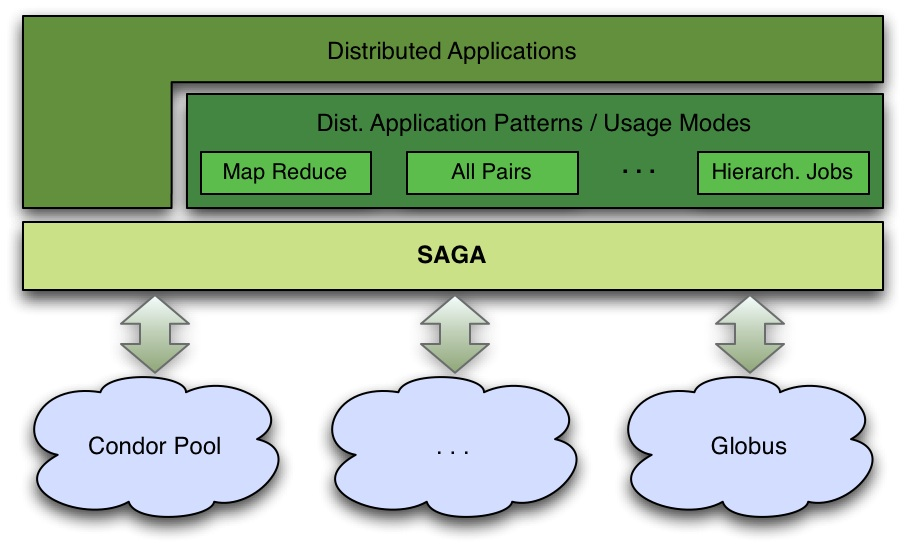
\includegraphics[width=8cm]{sagadistributedappslarge}
\caption{A distributed application running with SAGA, showing how SAGA insulates the application from the heterogeneous nature of multiple distributed resources (from SAGA web-site).}
\end{figure}

\begin{figure}
\centering	
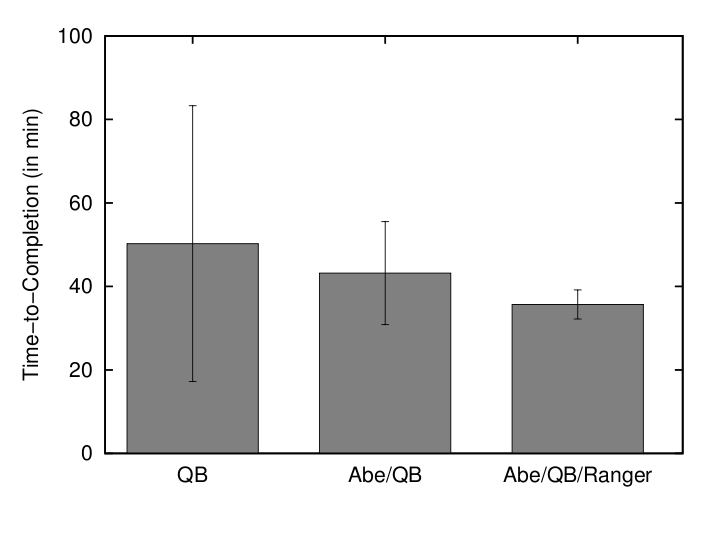
\includegraphics[width=6cm]{namd-rep-size-adaptive}
\caption{A comparison of average time to completion for SAGA/REMD NAMD on three sets of resources (Queen Bee, Abe + Queen Bee, Ranger + Abe + Queen Bee) when the number of processors is adjusted to fit the available resource at run-time.  Reproduced from \cite{ref:saganamd}.}
\end{figure}

\begin{figure}
\centering	
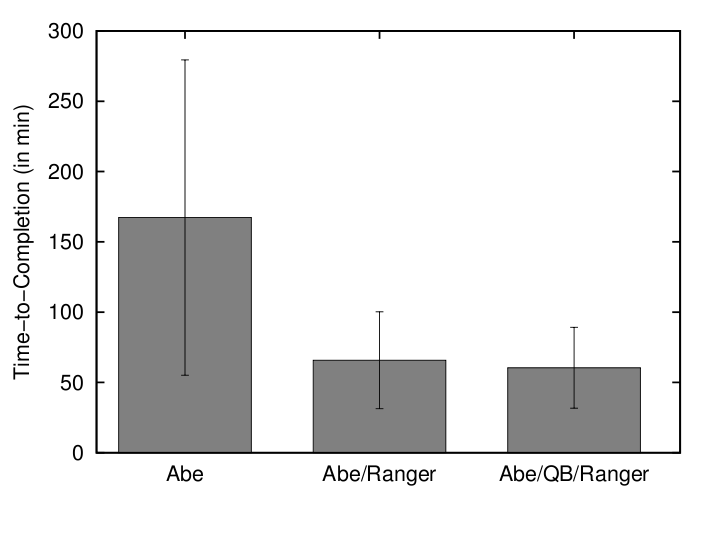
\includegraphics[width=6cm]{namd-rep-num-adaptive}
\caption{A comparison of average time to completion for SAGA/REMD NAMD on three sets of resources (Abe, Abe + Ranger, Ranger + Abe + Queen Bee) when the number of replicas is adjusted to fit the available resource at run-time.  Reproduced from \cite{ref:saganamd}.}
\end{figure}

\thispagestyle{plain}
\begin{thebibliography}{100}
\footnotesize


\bibitem{ref:hpdc} S. Manos, M. Mazzeo, O. Kenway, N. T. Karonis, B. Toonen and P. V. Coveney, Proceedings of High Performance Distributed Computing Boston, Massachusetts, USA, June 23-27 2008

\bibitem{ref:BAC} I. Stoica, S. K. Sadiq, and P. V. Coveney, Journal of the American Chemical Society, 130, (8), 2639-2648, 2008

\bibitem{ref:BAC2} S. K. Sadiq, D. Wright, S. J. Watson, S. J. Zasada, I. Stoica, Ileana, and P. V. Coveney, Journal of Chemical Information and Modeling, 48, (9), 1909-1919, 2008

\bibitem{ref:lammps} S. J. Plimpton, J Comp Phys, 117, 1-19 (1995)

\bibitem{ref:lammps2} S. J. Plimpton, R. Pollock and Mark Stevens, Proc of the Eighth SIAM Conference on Parallel Processing for Scientific Computing, Minneapolis (March 1997).

\bibitem{ref:saganamd} A. Luckow, S. Jha, J. Kim, A. Merzky, B. Schnor,  Phil. Trans. R. Soc. A 28 June 2009 vol. 367 no. 1897 2595-2606

\bibitem{ref:saganamd2} A. Luckow, S. Jha, J. Kim, A. Merzky, B. Schnor,  escience, pp.253-260, 2008 Fourth IEEE International Conference on eScience, 2008

\bibitem{ref:namd} J. C. Phillips, R. Braun, Wei Wang, J. Gumbart, E. Tajkhorshid, E. Villa, C. Chipot, R. D. Skeel, L. Kale, and K. Schulten, Journal of Computational Chemistry, 26:1781-1802, 2005.

\end{thebibliography}

\thispagestyle{plain}
\end{document} 